\subsection{2D Plots of ISVD with Varying Number of Eigenvalue} \label{sec:isvdCompare2d}
\begin{figure}[H]
    \centering
    \subfloat[\centering Using $1$ Eigenvalue]
    {{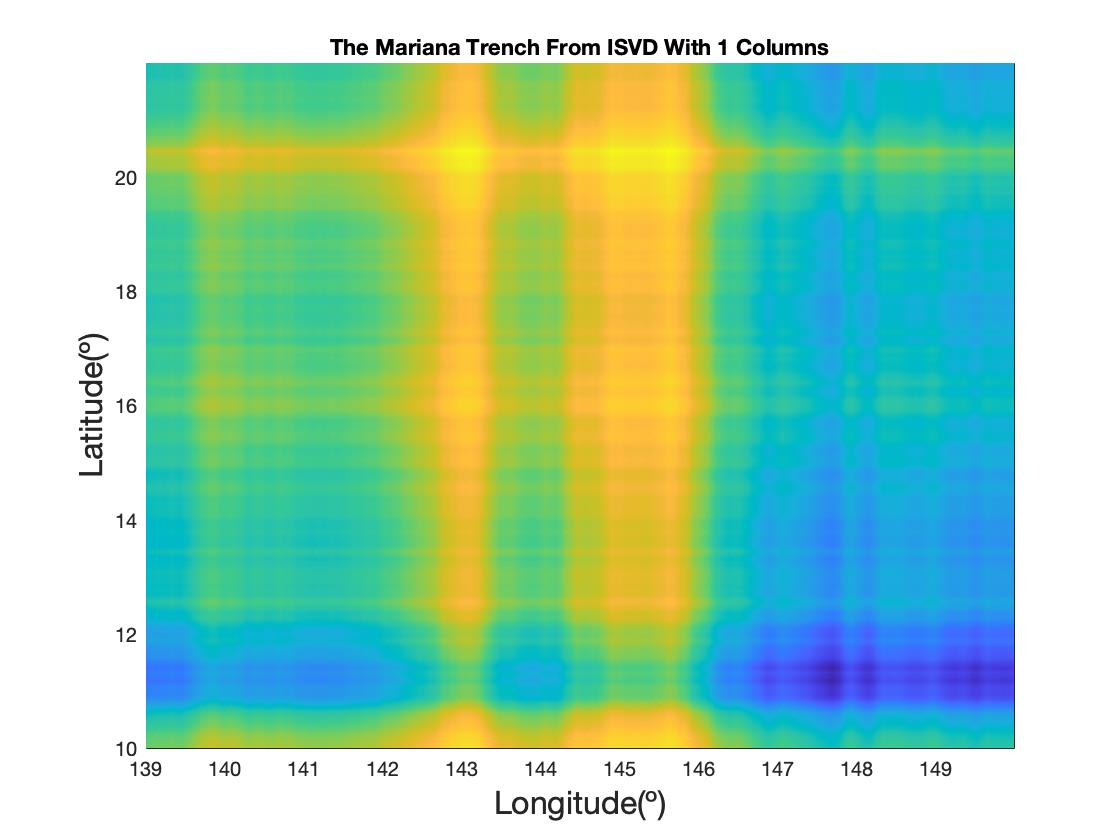
\includegraphics[width=0.45\textwidth]{./imgs/twoD1Col.jpg}}}%
    \qquad
    \subfloat[\centering Using $10$ Eigenvalues]
    {{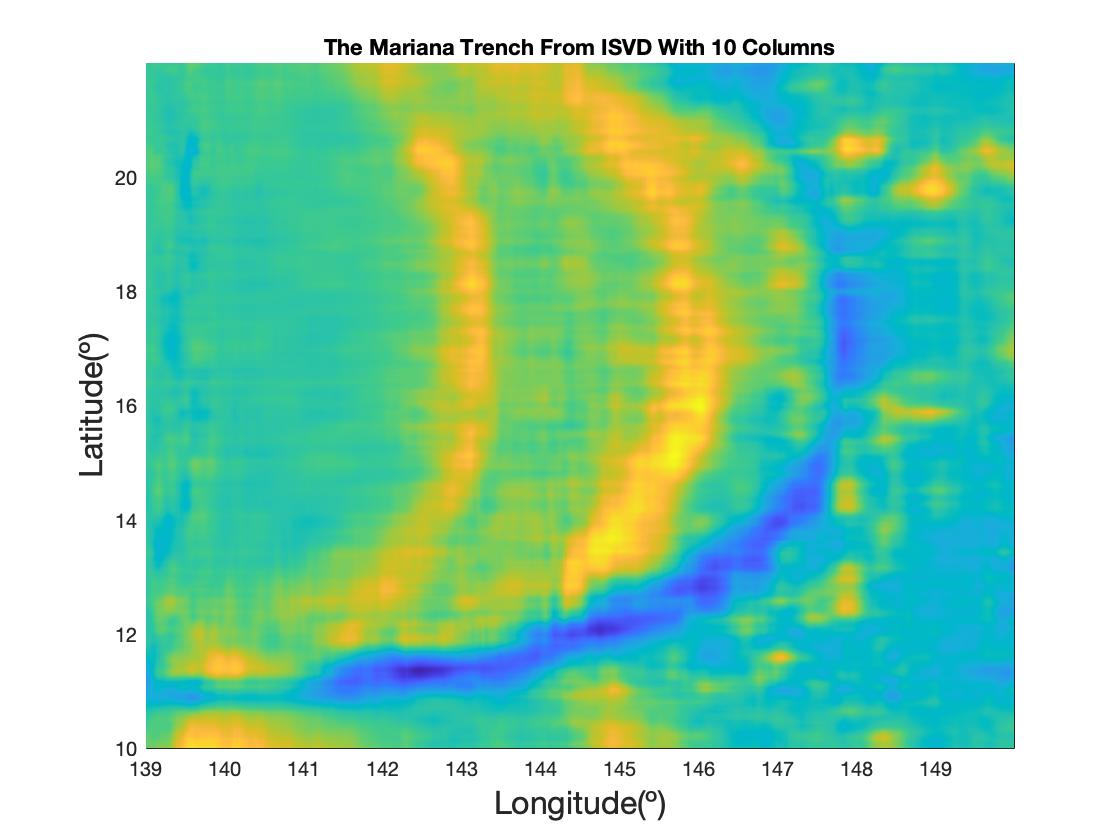
\includegraphics[width=0.45\textwidth]{./imgs/twoD10Col.jpg}}} \\
    \subfloat[\centering Using $100$ Eigenvalues]
    {{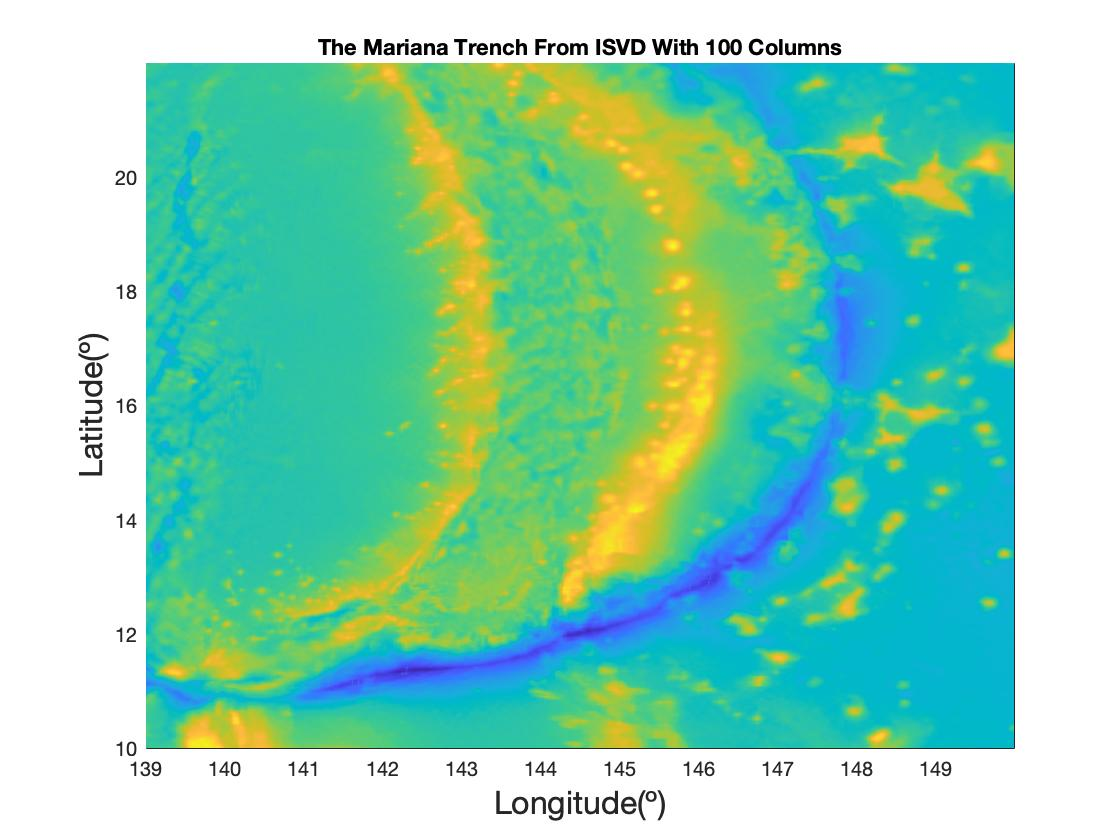
\includegraphics[width=0.45\textwidth]{./imgs/2D100Col.jpg}}}%
    \qquad
    \subfloat[\centering Using $500$ Eigenvalues]
    {{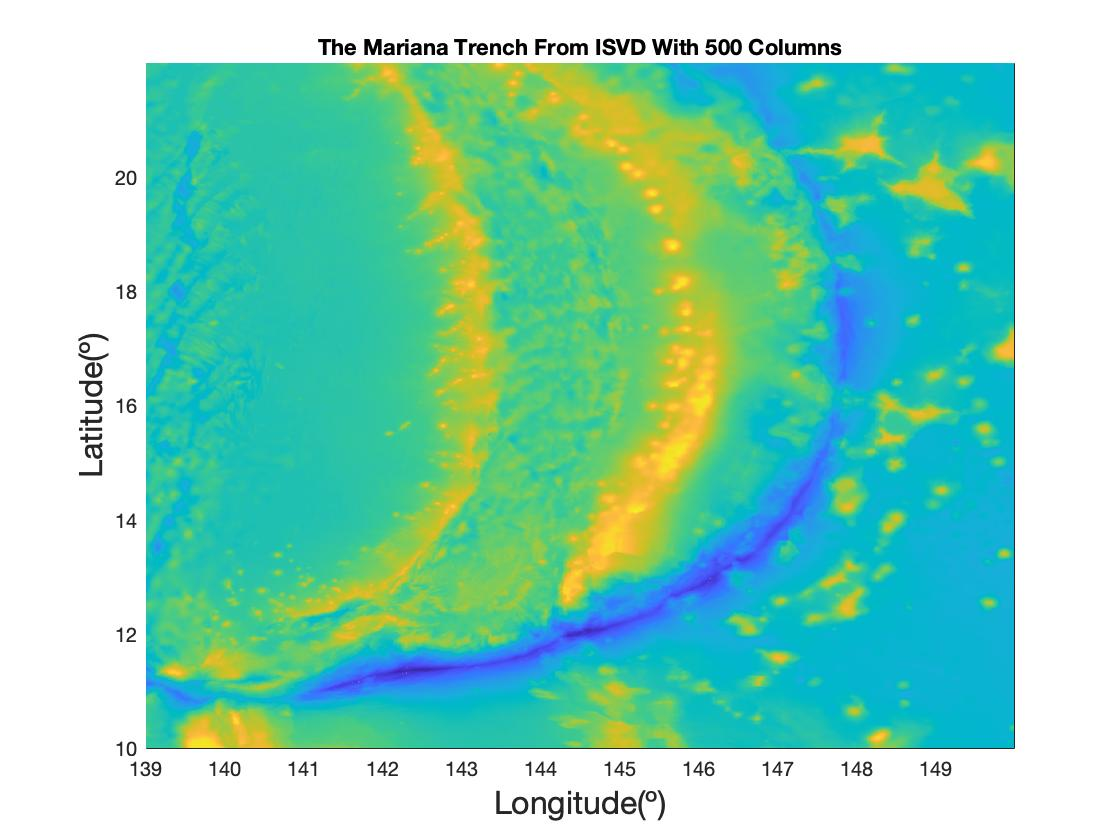
\includegraphics[width=0.45\textwidth]{./imgs/2D500C0l.jpg}}}%
    \caption{2D Plots of ISVDs Using Different Numbers of Eigenvalues for Comparison}%
    \label{fig:comparison2D}%
\end{figure}